
\documentclass{article}
\usepackage[utf8]{inputenc}
\usepackage[bulgarian]{babel}

\usepackage{systeme}
\usepackage{amsmath}

\usepackage{cmap}
\usepackage[utf8]{inputenc}
\usepackage[T2A]{fontenc}

\newtheorem{definition}{Дефиниция}

\usepackage{comment}
%\use
\newtheorem{problem}{Задача}

\newcounter{solution}

\usepackage{graphicx}

\newcommand\solution{%
	\stepcounter{solution}%
	\textbf{Решение :}\\%
}


\date{}

\title{Книжка за упражнителни задачки на Деспина}
\begin{document}
	
	
	\maketitle
	
	
	\section{Теория}
	
	\subsection{Триъгълник}
	
	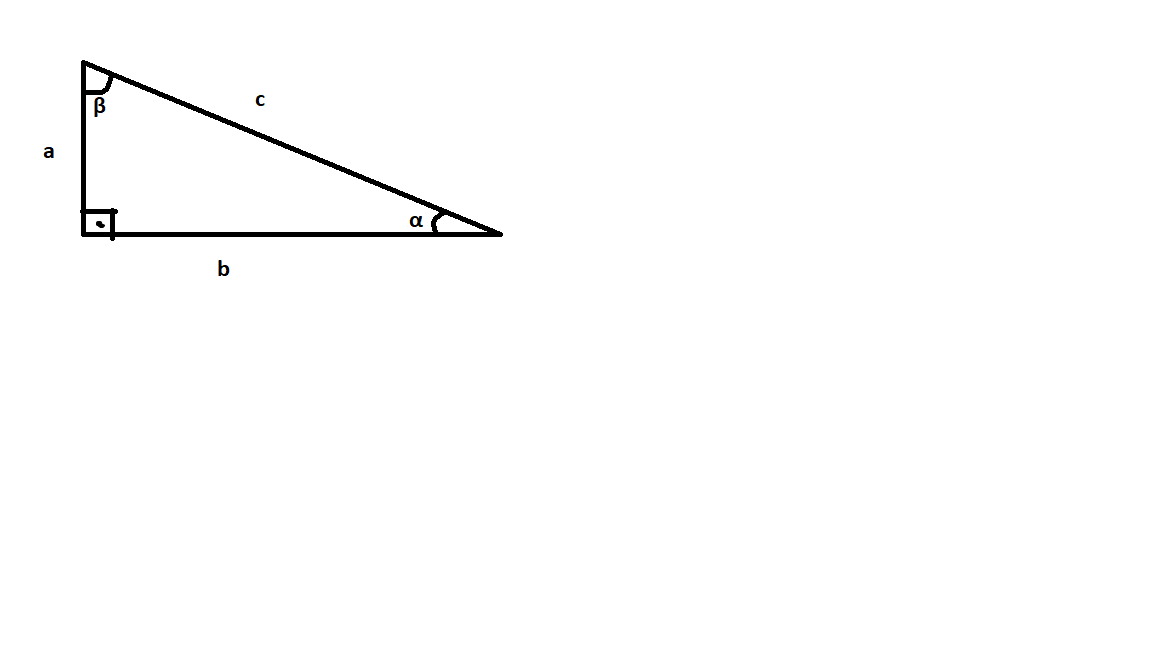
\includegraphics{Trig1}
	
	\vspace{-8cm}
	
	\begin{definition}$ sin(\alpha) = \frac{a}{c} $, $ cos(\alpha) = \frac{b}{c} $, $tg(\alpha) = \frac{a}{b} $, $cotg(\alpha) = \frac{b}{a} $	
	\end{definition}
Да зебележим, че $ sin(\beta) = cos(\alpha) = \frac{b}{c} $ и аналогично $cos(\beta) = sin(\alpha ) = \frac{a}{c} $.
$a^2 + b^2 = c^2  \to (\frac{a}{c})^2 + (\frac{b}{c})^2 = 1 \to sin^2(\alpha) + cos^2(\alpha) = 1$. \\
Тригонометрични тъждества ($\alpha, \beta \in [0,90] )$: \\
$sin^2(\alpha) + cos^2(\alpha) = 1$ \\
$ sin(\alpha) = cos(\beta) = cos(90 - \alpha) $ \\
$ tg(\alpha)cotg(\alpha) = 1 $ \\
$ tg(\alpha) = \frac{a}{b} = \frac{a}{c} \cdot \frac{c}{b} = \frac{sin(\alpha)}{cos(\alpha)} $, $cotg(\alpha) = \frac{1}{tg(\alpha)} = \frac{cos(\alpha)}{sin(\alpha)} $ 

\begin{problem}
	Да се намерят останалите тригонометрични функции, ако $cos(\alpha) = 0.3 $
\end{problem}
\solution
$sin^2(\alpha) + cos^2(\alpha) = 1 \to sin^2(\alpha) = 1 - 0,09 \to sin(\alpha) = \sqrt{0,91}  $  \\
$tg(\alpha) = \frac{\sqrt{0,91}}{0,3} = \frac{10\sqrt{0,91}}{3} $ \\
 $cotg(\alpha) = \frac{0,3}{\sqrt{0.91}} = \frac{3}{10} \cdot \frac{\sqrt{0,91}}{0,91} = \frac{30\sqrt{0,91}}{91}  $
\begin{problem}
	Да се намерят останалите тригонометрични функции, ако $cos(\gamma) = \frac{\sqrt2}{2} $, $cos(\alpha) = \frac{1}{2} $.
\end{problem}
\solution $cos(\alpha) = \frac{1}{2} \to sin^2(\alpha) = 1 - \frac{1}{4} = \frac{3}{4} \to \sqrt{sin^2(\alpha)} = \sqrt{\frac{3}{4}} $ \\
$ sin(\alpha) = \frac{\sqrt3}{\sqrt4} = \frac{\sqrt3}{2} $ \\
$ tg(\alpha) = \frac{\frac{\sqrt3}{2}}{\frac{1}{2}} = \sqrt{3} $ \\
$cotg(\alpha) = \frac{1}{\sqrt3} = \frac{\sqrt3}{\sqrt9} =  \frac{\sqrt3}{3}$




\subsection{Вероятности - Комбинации, Вариации и Пермутации.}

\begin{definition}
	Пермутации - начини, по които може да наредим $n$ обекта в една линия.
\end{definition}
Пример. Пермутация от 3 елемента са начините, по които може да наредим 3 "неща" на една линия едно до друго. Нека за определеност да са молив, химикал и флумастер. Начините, по които може да ги наредим са: \\
ФХМ, ФМХ, МХФ, МФХ, ХМФ, ХФМ или общо 6 начина. Нека да добавим 4ти елемент ролер. За първото нареждане ФХМ, ролерът може да е на 4 позиции:
РФХМ, ФРХМ, ФХРМ, ФХМР. Тогава 4те елемента може да ги наредим по 6.4 = 24 начина. $n$ обекта могат да се наредят по $n(n-1)...1$ начина. 
Примерите по горе Ф, Х и М могат да се наредят по $3.2.1 =6 $ начина и Ф,Х, М, Р могат да се наредят по $4.3.2.1 = 24$ начина. Дефинираме $n$-факториел с $n! = n(n-1)...1$.


\begin{definition}
Вариация - избор на елементи където реда има значение - Налучкване на телефонен номер. $V_{10}^4$.
\end{definition}


\begin{definition}
	Комбинации - избор на елементи където реда няма значение - начини за вземане на различни цветове топки от урна(напр. сини, червени, зелени, жълти и т.н.).
\end{definition}

\begin{problem}
По колко начина може да изберем 6 молива(различни) 10 молива(различни)?(Реда няма значение).
\end{problem}
\solution Първи молив избираме по 10 начина, втория - по 9, и т.н. Общо 10.9.8.7.6.5 начина.



\begin{problem}
	Дадени са 10 молива с различни цветове. За оцветяване на картинка са необходими 6 точно определени цвята. Каква е вероятността случайно избрани 6 молива да могат да оцветят картинката?
\end{problem}
\solution
Вероятността първия молив да е от 6те е $\frac{6}{10}$. Вероятността втория молив да е подходящ за оцветяване е  $\frac{5}{9}$ и т.н. Вероятността от 6 тегления да изтеглим моливите за оцветяване е $\frac{6.5.4.3.2.1}{10.9.8.7.6,5} = \frac{3}{10.9.7} = \frac{1}{10.3.7} = \frac{1}{210}$. \\
За упражение: 2 молива от 3.




	\section{Входно ниво 10ти клас}
	
	\section{Kвадратни уравнения и системи}
	
		
	\begin{enumerate}
		\item системи уравнения
		\item квадратни уравнения
		\item неравенства (???)
		\item други уравнения
	\end{enumerate}
	
	
	
	Фромули, които се изпозлват за квадратни уравния: \\
	Ако е дадено уравнение $ax^2 + bx + c = 0  $, имаме дискриминанта  $ D= b^2 - 4ac $, тогава решенията се задават с $ x_{1,2} = \frac{-b \pm \sqrt{D}  }{2a}$. Да разгледаме еднин пример. 
	Упражение(?): $(x - \frac{-b + \sqrt{D}  }{2a}  )(x - \frac{-b - \sqrt{D}  }{2a}) = ax^2 + bx +c $

	
	Припомняме формулите за съкратено умножение:\\
	 $(a+b)^2 = a^2 + 2ab + b^2$ \\
	 $(a-b)^2 = a^2 - 2ab + b^2$ \\
	 $(a+b)(a-b) = a^2 - b^2 $
	 
	 \vspace{1cm}
	 
	 
	
	Упражнителни задачи, които Деспина е решавала сама: \\
	
		$$x^2 - 5x + 6 = 0$$  \\
		
		
		\vspace{3cm}
		
		Още примери за решаване: \\
		\begin{enumerate}
			\item $x^2 - 6x + 8 = 0$
			\item $x^2 - 5x + 6 = 0$
			\item $x^2 - 5x + 6 = 0$
			\item $x^2 - 5x + 6 = 0$
			\item $x^2 - 5x + 6 = 0$
			\item $x^2 - 5x + 6 = 0$
		\end{enumerate}

		
		
		\newpage
	\section{Еднаквост и подобност на триъгълници}	
	
	Важно! Един триъгълник се определя от "три неща" - 
	три страни, две страни и ъгъл между тях, страна и два ъгъла. \\
	
	
	Признаци за еднаквост:
	\begin{enumerate}
		\item две страни и ъгъл между тях = две страни и ъгъл между тях $=>$  еднакви
		\item страна и два ъгъла = страна и два ъгъла $=>$  еднакви
		\item три страни = три страни $=>$ $ $ еднакви
	\end{enumerate}

	\vspace{1cm}
	
	
	Важно! Подобните триъгълници си приличат по това, че имат една и съща форма, но единият е 10 пъти или 5 пъти(или колкото и да е пъти) "по-голям" от другия \\
	
		Признаци за подобност:(Трябва да се потвърди от учебник)
	\begin{enumerate}
		\item (???) две страни са 5 пъти по-малки и ъгълът между тях е равен.
		\item (???) една страна е 5 пъти по-малка и 2 ъгъла са равни.
 		\item  (???) трите ъгъла са равни
 	\end{enumerate}
	
	
	
	\vspace{2cm}
	ирационални изрази, прогресии, статистика и обработка на данни, 
	решаване на триъгълник- sin, cos, tg, cotg в (0,180), синусова и косинусова теорема (?), елементи от стереометрията
	
		

\section{Тригонометрия}


\section{Задачи с текс}

\subsection{Разни}


\subsection{Линейни уравнения и неравенства}

\begin{problem}
	Сборът на две последователни естествени числа е със 131 по-малък от произведението им. Намерете числата.	
\end{problem}
\solution
 Ако първото(по-малкото от двете числа е $x$), второто число е $x+1$. Тогава от условието на задачата имаме 
 $ x + x+1 = x(x+1) - 131 $ \\ $2x + 1 = x^2 + x - 131.$ \\
 $x^2 + x - 131  -2x -1 = 0.$ \\
 $ x^2 -x -132 = 0.$
$D = (-1)^2 - 4.(-132) = 1 + 4.132 = 528+1 =529.$
$x_1 = \frac{1 +23}{2} = 12 $ . $x_2 = \frac{1 - 23}{2} = -11$. $-11$ не е естествено.
Отг. $12$ и $13$.

\begin{problem}
	В един магазин продали 488 кг портокали, лимони и маслини. Портокалите били с 40 кг повече от лимоните, а маслините - 5 пъти по-малко от портокалите. По колко килограма са продали от всеки вид?
\end{problem}

\begin{problem}
	През един сезон в консервната фабрика "Добруджанка" са обработили по 48 т домати на ден. След като предали 1300 т пресметнали, че това е с 524тт по-малко от цялото количество домати. Колко дни въъв фабриката са обработвани домати?
\end{problem}


\begin{problem}
	Обиколката на един триъгълник е 126 см. Едната му страна е с 12 см по-къса от другата , а третатат е 3/ от сбора на првите две. Да се намери най--голямата страна на този триъгълник.
\end{problem}


\begin{problem}
	Попитали Николай на колко е години, а той отговорил: "Мама е на 38 години. Тя е с 2 години по-млада от татко. Татко пък има два пъти повче години, отколкото аз и сестра ми заедно. Но аз със с 4 години по-малък от сестра ми." На коолко години са Николай и сестра му?
\end{problem}


\begin{problem}
	Един работник може да свърши определена работа за 15 дни, а друг работник за същото време свършва само 75 \% от тази работа. Отначало ддвамата  работници работели заедно 6 дни, а след това вторият само довършил останалата част. За колко дни била свършена цялата работа и какъв процент от нея е изработил всеки един работник?
\end{problem}

\subsection{Басейни}

\begin{problem}
	Един басейн се пълни от една тръба за 2 ч, от друга за 3ч, от трета за 4ч. За колко време се пълни от трите едновременно? 
\end{problem}


\begin{problem}
	Един басейн се пълни от една тръба за 2 ч, от друга за 3ч. За колко време се пълни от двете едновременно? Каква част пълни всяка от тръбите?
\end{problem}

\solution
Разсъждения. За 1 час пълним $\frac{1}{2} + \frac{1}{3} = \frac{3}{6} + \frac{2}{6} = \frac{5}{6}$. Тогава ако времето за пълнене е $x$(в часове), то $\frac{x}{2} + \frac{x}{3} = 1 $. Тогава $3x + 2x = 6 $ и  $ x = \frac{6}{5}$ часа или 1ч и 12мин. Първата тръба е напълнила $\frac{1}{2}\cdot \frac{6}{5} = \frac{3}{5} = 60\% \cdot $. Тогава втората е напълнила $\frac{2}{5} = 40\%$ от басейна.
 
(Koментар: Първия басейн пълни за минута $\frac{1}{120}$, а втория $\frac{1}{180}.$ За $12$ минути пълним $\frac{12}{120} + \frac{12}{180} = \frac{12.3 + 12.2}{360} = \frac{60}{360} \cdot \frac{1}{6}. )$


\begin{problem}
	Един басейн се пълни от една тръба за 10ч, а от друга за 12ч. Първата тръба е пълнила 1 час, след което е спряла за 30 минути ремонт, след това е продължила да пълни. Втората тръба работи безотказно. За колко време двете тръби заедно напълват басейна.
\end{problem}
\solution 
 Нека с х означим времето за пълнене. За 1ч имаме напълнено $\frac{1}{10} + \frac{1}{12} = \frac{12}{120} + \frac{10}{120} = \frac{22}{120} \cdot$. За следващия половин час пълни само втората тръба, т.е. за времето между 1ч и 1ч и 30 минути пълним $\frac{1}{12} \frac{1}{2} = \frac{1}{24}.$ Остава ни да напълним $1 - \frac{22}{120} - \frac{1}{24}.$ Ако означим оставащото време с $y$, то за $y$ имаме $ \frac{y}{10} + \frac{y}{12} =  1 - \frac{22}{120} - \frac{1}{24}$. Сумарното време за пълнене е $y+1+\frac{1}{2}$. Остава да намерим $y$.



\begin{problem}
	Един басейн се пълни от една тръба за 10ч, а от друга за 12ч. Първата тръба е пълнила 1 час, след което е спряла за 1 ремонт, след това е продължила да пълни. Втората тръба работи след 1вия час. За колко време се напълва басейна?
\end{problem}




\section{Системи}

\begin{problem}
	\[
	\begin{cases}
	x - y = 7 \\
	x^2 - xy - y^2=19 \hspace{2cm} x = y + 7 
	\end{cases}
	\]
\end{problem}

\noindent
\solution
$ x = y + 7 $ \\
$ (y+7)^2 - (y+7)y - y^2 = 19 $ \\
$ y^2 + 14y + 49 - y^2 - 7y - y^2 = 19 $ \\
$ -y^2 + 7y + 30 = 0 $ \\ 
$ y^2 - 7y - 30 = 0  \to a = 1, b = -7 , c = -30$ \\ 
$D = 49 + 120 = 169, y_1 = 10$ , $y_2 = -3 $ \\
$x_1 = 10 + 7 = 17, x_2 = -3 + 7 = 4$ \\
Отг. Решенията на системата са: $(17,10) , (4,-3)   $

\vspace{1cm}

\begin{problem}
	\[
	\begin{cases}
	2x - y -1 = 0 \\
	xy - 1 = 0  
	\end{cases}
	\]
\end{problem}
\solution
$ y = 2x -1$ \\
$ x(2x-1) - 1 = 0 $ \\
$ 2x^2 - x - 1 = 0 \to a=2, b = -1, c= -1$  \\
$ D = 1 - 4.2.(-1) = 9 $
$ x_1 = \frac{-(-1)+ \sqrt{9}}{2.2}= \frac{4}{4} = 1 $, $x_2 = \frac{-(-1)- \sqrt{9}}{2.2}= -\frac{2}{4} = -\frac{1}{2}  $
$ y_1 = 2x_1 - 1 = 2 - 1 = 1 $, $y_2 = 2x_2 - 1 = 2(-\frac{1}{2})-1 = -2  $ \\
Отг. $(1,1), (-\frac{1}{2}, -2  ) $

\begin{problem}
	\[
	\begin{cases}
	x + y = -2 \\
	x^2 + y^2 = 2 
	\end{cases}
	\]
\end{problem}

\begin{problem}
	\[
	\begin{cases}
	x - 3y + 1 = 0 \\
	x^2 - 4xy + 3y^2 + x - y = 0 
	\end{cases}
	\]
\end{problem}



\section{Ирационални уравнения}

\begin{problem}
	Решете уравнението: $\sqrt{x - 5} -  \sqrt{20-x} = -1  $
\end{problem}
\solution  $\big(\sqrt{x - 5} -  \sqrt{20-x}  \big)\big(\sqrt{x - 5} +  \sqrt{20-x}  \big) = x+5 + 20 - x  = 25 \to$ няма решение.


\begin{problem}
	Решете уравнението: $\sqrt{x - 2} -  \sqrt{2x-1} = 0  $
\end{problem}
\solution  $(\sqrt{x - 2} -  \sqrt{2x-1} )(\sqrt{x - 2} +  \sqrt{2x-1}) =  x-2 +2x - 1 = 3x - 3   
$ \\
$ 3x = 3 \to x = 1 $. \\
 Проверка:
$\sqrt{1 - 2} -  \sqrt{2-1} = \sqrt{-1} - \sqrt{1} \neq 0 \to $ няма решение. \\
За другия път $x - 2 \geq 0 $ и $ 2x-1 \geq 0 $
\begin{comment}

\begin{align*}
x &= a^{\log_a (x)} \bigg\vert \ln () \\
\Leftrightarrow \qquad \ln (x) &= \ln \left(a^{\log_a (x)} \right) \\
\Leftrightarrow \qquad \ln (x) &= \log_a (x) \cdot \ln (a) \bigg\vert - \ln (a) \\
\Leftrightarrow \qquad \frac{\ln (x)}{\ln (a)} &= \log_a (x) 
\end{align*}

\begin{align*}
&\left\{
\begin{aligned}
I_{50}+I_{10}=I_{03}\\
I_{21}=I_{12}+I_{10}\\
I_{12}+I_{32}=I_{21}\\
I_{03}=I_{32}+I_{34}\\
I_{34}=I_{451}+I_{452}\\
\end{aligned}\right.
&
\left\{\begin{aligned}
U_{30}+U_{01}+U_{121}+U_{23}=0\\
U_{34}+U_{452}+U_{50}+U_{30}=0\\
U_{121}+U_{122}=0\\
U_{451}+U_{452}=0\\
\end{aligned}\right. \\
&\text{, pentru legea I, și}
&\text{pentru legea a II-a}
\end{align*}

\end{comment}



\end{document}	
	
	

